\documentclass[11pt,a4paper]{article}
\usepackage[hyperref]{acl2023}
\usepackage{graphicx}
\usepackage{float}
\usepackage{caption}
\usepackage{tcolorbox}
\usepackage{subcaption}
\usepackage{amsmath} 
\usepackage{amsfonts}
\tcbuselibrary{skins, breakable}
\tcbuselibrary{listings, breakable}

\title{
    Multi-Class Classification and Denoising of EEG Artifacts Using the Wearable BART Headset\\
    \large Laboratory of Wearable Biosignal Processing, Academic Year 2025-26
}
\author{
    Christian Prendin\\
    \texttt{christian.prendin@mail.polimi.it}
    \AND
    Mirko Pica\\
    \texttt{mirko.pica@mail.polimi.it}
    \And
    Jakub Rymarski\\
    \texttt{jakub.rymarski@mail.polimi.it}
}
\date{June 2026}

\begin{document}

\maketitle

\begin{abstract}
High-amplitude physiological and motion artifacts pose a fundamental challenge for low-density, wearable electroencephalography (EEG). This work presents a complete pipeline for multi-class artifact classification and denoising on a 4-channel temporal headset (BART) across 13 subjects, targeting seven categories: eye blinks, leftward and rightward saccades, jaw clenches, horizontal and vertical head movements, and resting baseline. Under strict Leave-One-Subject-Out (LOSO) cross-validation, a four-stage hierarchical XGBoost architecture operating on a 324-dimensional handcrafted feature space achieved the best chained macro F1 of 0.658, outperforming Random Forest (0.620), EEGNet (0.571), and a 1D-CNN (0.620). Deep networks were structurally constrained by the limited spatial density of the 4-channel configuration. The primary bottleneck across all models was Stage 3b discrimination of horizontal versus vertical head movements, which proved indistinguishable at frontal-temporal electrode positions. For artifact suppression, four methods were benchmarked against per-subject rest baselines: Discrete Wavelet Transform (DWT), Artifact Subspace Reconstruction (ASR), a cascaded DWT-ASR pipeline, and a residual 1D convolutional autoencoder. ASR and the cascade provided the most consistent broadband suppression. The autoencoder achieved superior artifact-band attenuation on ocular deflections but failed on jaw clench due to a spectral mismatch between its learned subtraction template and broadband EMG content.
\end{abstract}

\begin{figure}[h]
    \centering
    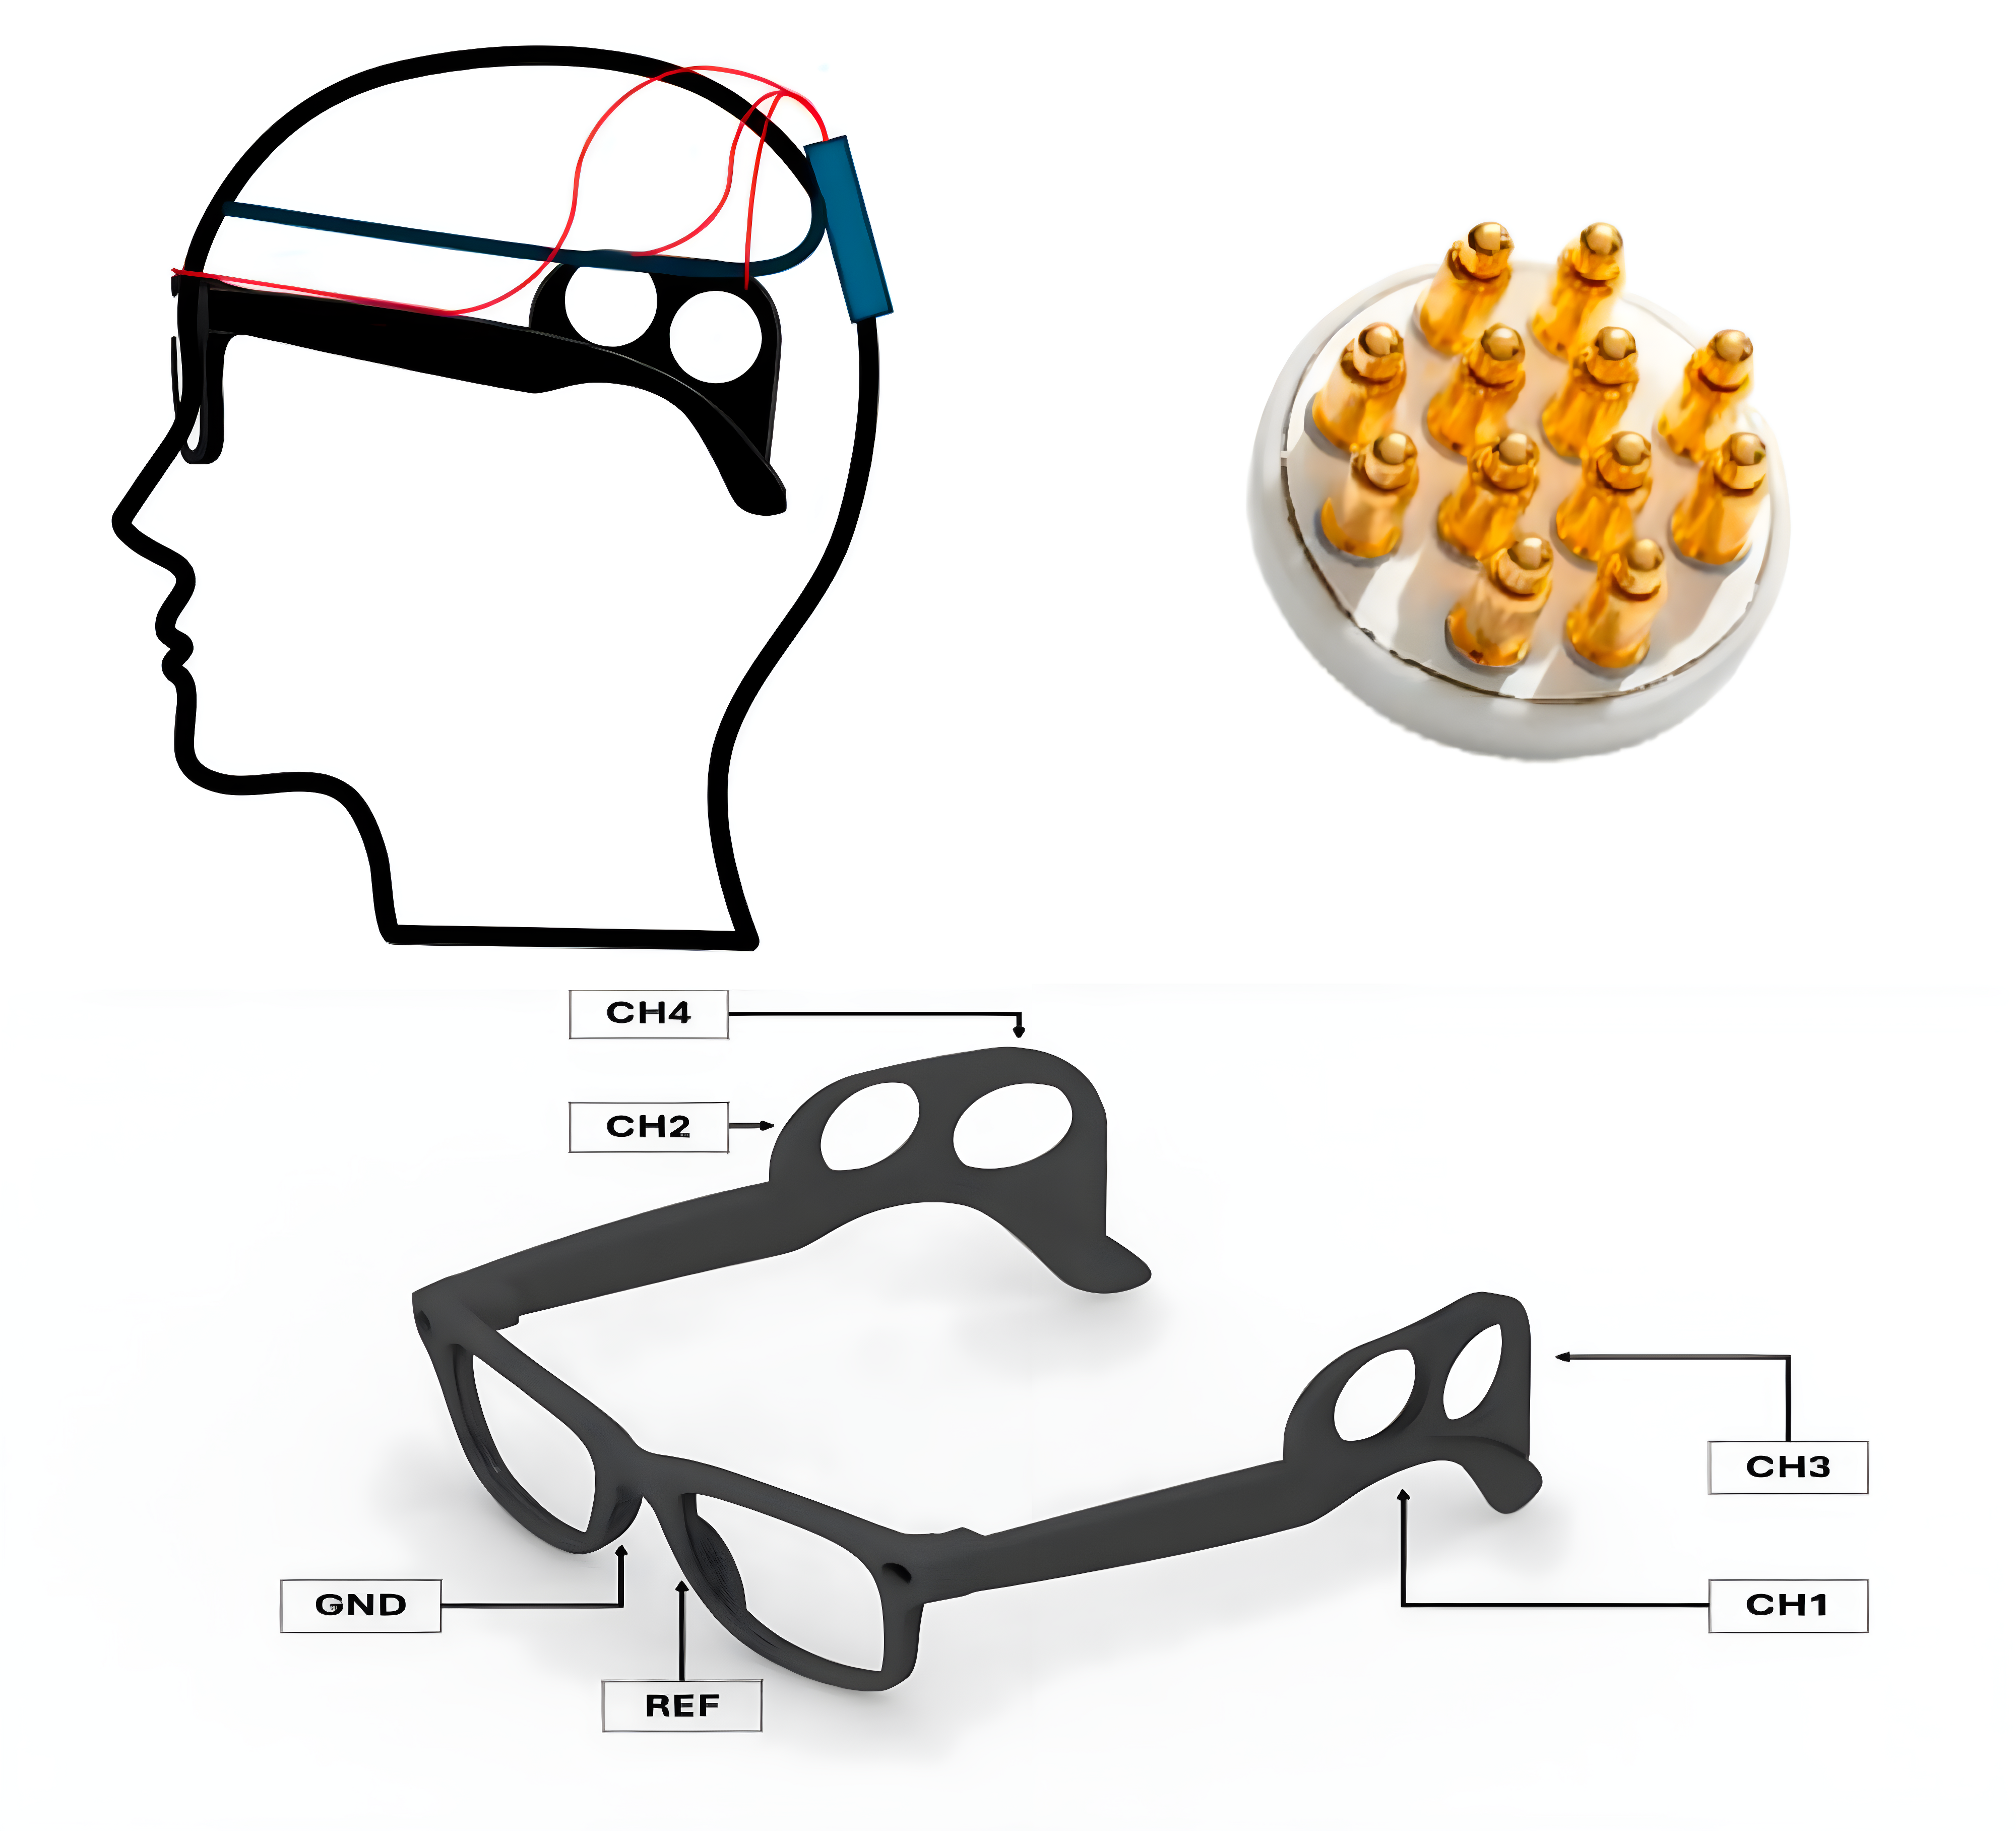
\includegraphics[width=0.85\columnwidth]{figures/bart.png}
    \caption{BART device.}
    \label{fig:bart}
\end{figure}

\section{Introduction}
The translation of electroencephalography (EEG) from electromagnetic-shielded laboratories to ambulatory clinical and consumer domains is primarily constrained by signal vulnerability to exogenous interference. Low-density, dry-electrode systems like the portable BART headset improve patient compliance and logistical mobility, but their unshielded configuration exacerbates sensitivity to high-amplitude physiological and mechanical artifacts. Ocular dipoles during blinks or saccades distort frontal traces, while cranial muscular contractions introduce high-frequency electromyographic (EMG) bursts that overwhelm microvolt-level cortical potentials; direct epoch rejection compromises temporal continuity and data integrity in real-time brain-computer interfaces (BCIs).

This work presents a complete artifact management pipeline for the 4-channel BART headset, evaluating a four-stage hierarchical classifier against a rule-based thresholding baseline and benchmarking four artifact suppression methods, all under strict Leave-One-Subject-Out (LOSO) cross-validation across 13 subjects.

\section{Experimental Protocol \& Data Acquisition}

\subsection{Hardware Configuration and Electrode Mapping}
Biopotential data acquisition was conducted using the BART wearable EEG system, an ultra-portable, glasses-style rigid frame with four active recording channels (CH1--CH4) using dry, gold-plated electrodes. Hardware reference (REF) and ground (GND) nodes are integrated into the nasal bridge.

The four sensors are mounted bilaterally along the temple arms, approximating the T3/T4/T5/T6 positions of the international 10--20 system 
(Figure~\ref{fig:1020}):
\begin{itemize}
    \item \textbf{Anterior pair (CH1, CH2):} Anterior to the ear; sensitive to the corneal-retinal dipole variations produced by eye blinks and horizontal saccades.
    \item \textbf{Posterior pair (CH3, CH4):} Slightly posterior to the ear, near the temporalis and masseter muscles; captures EMG bursts during jaw clenches and mechanical vectors from gross head movements.
\end{itemize}
This lateral temporal placement lacks the spatial specificity required to distinguish horizontal from vertical head rotation, a fundamental hardware constraint discussed in Section~\ref{sec:discussion}.

\begin{figure}[h]
    \centering
    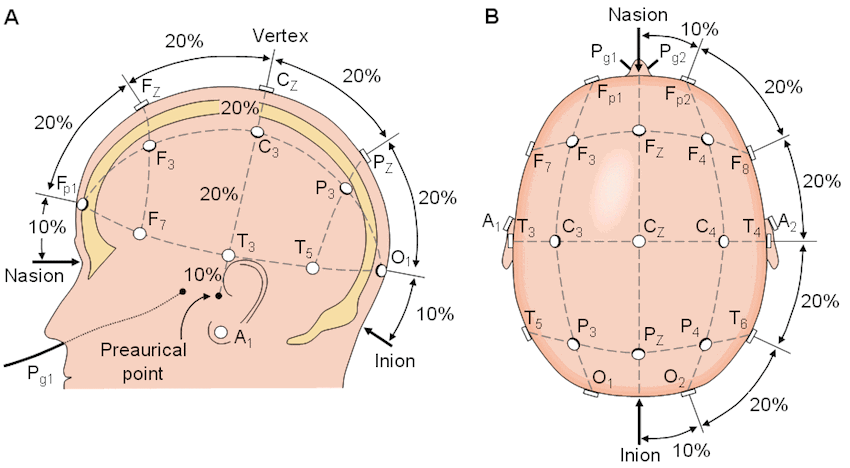
\includegraphics[width=0.85\columnwidth]{figures/1020.png}
    \caption{International 10--20 system.}
    \label{fig:1020}
\end{figure}

\subsection{Subject Pool and Pre-Session Calibration}
The cohort comprised 13 university subjects. Before each recording block, electrode contact and frame seating were verified, live signal quality was inspected for drift or saturation, LSL marker synchronization was confirmed, and subjects completed one unrecorded practice trial.

\subsection{Timeline and Trial Structure}

The paradigm used a cross-randomized block design lasting approximately 10~minutes per subject, illustrated in Figure~\ref{fig:protocol}. Each session was anchored by a fixed rest block (two 60-second sub-blocks: Eyes Open then Eyes Closed) at both start and end. Between these anchors, six active artifact blocks of 40 seconds each (Blinks, Leftward Saccades, Rightward Saccades, Jaw Clenches, Horizontal Head Movements, and Vertical Head Movements) were presented in randomized order, followed by a final, fixed 40-second Mental Arithmetic block. All active blocks were separated by 10-second transitional pauses.

\begin{figure}[h]
    \centering
    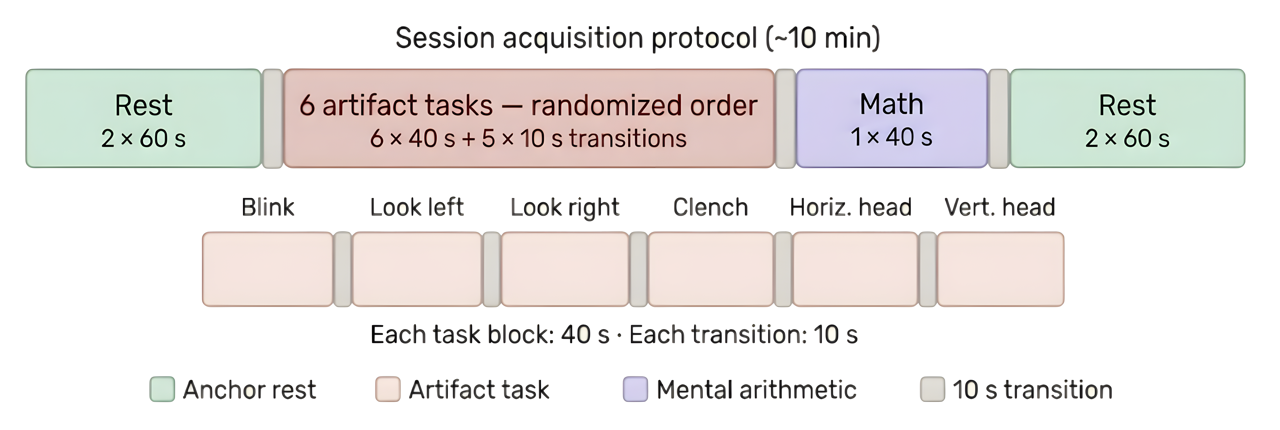
\includegraphics[width=\columnwidth]{figures/eeg_acquisition_protocol.png}
    \caption{Session timeline.}
    \label{fig:protocol}
\end{figure}

\subsection{Ground Truth Annotation and Window Extraction}
Synchronized event markers were injected into the LSL stream at each block boundary, defining the ground-truth label for all windows within that block. The continuous signal was segmented into 2-second sliding windows (500 samples at 250~Hz) with a 75\% overlap (0.5~s step), producing 11{,}418 labelled windows across 13 subjects. No window was permitted to span a block boundary. The first 10~seconds of each Eyes Closed sub-block were reserved for normalisation calibration (Section~\ref{sec:preprocessing}) and excluded from the labelled dataset to prevent leakage.

\subsection{Exploratory Data Analysis}
\label{sec:eda}
Prior to classifier training, exploratory analysis confirmed a distinct morphological and spectral split between artifact types (Figure~\ref{fig:blink_std_eda} and Figure~\ref{fig:blink_psd_eda}). Time-domain statistics revealed that eye blinks produce impulsive, high-kurtosis deflections, whereas jaw clenches and head movements exhibit sustained, high-energy amplitudes. Spectrally, ocular and head motion artifacts concentrate power in the low-frequency delta--theta range, while jaw clenches display broadband elevation in the gamma band, particularly on posterior channels.

\begin{figure}[h]
    \centering
    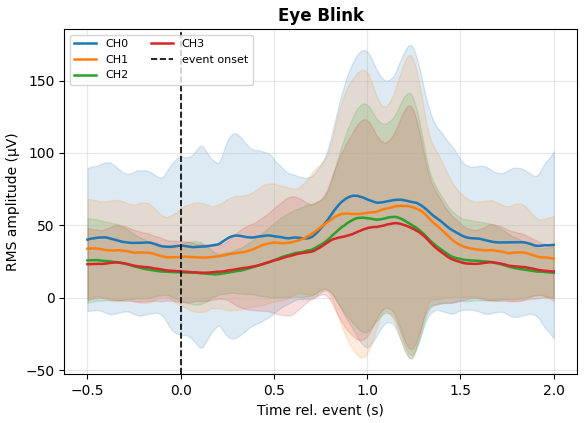
\includegraphics[width=\columnwidth]{figures/Blink_STD.png}
    \caption{Mean RMS amplitude envelope per artifact class across all channels and subjects.}
    \label{fig:blink_std_eda}
\end{figure}

\begin{figure}[h]
    \centering
    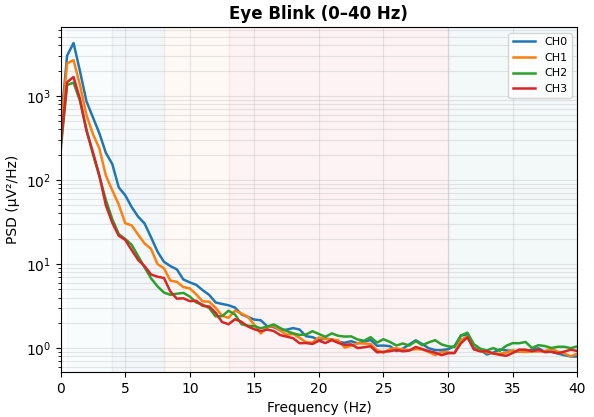
\includegraphics[width=\columnwidth]{figures/Blink_PSD.png}
    \caption{Welch PSD on Blinks artifacts — All Channels Overlaid (mean across subjects).}
    \label{fig:blink_psd_eda}
\end{figure}

\section{Signal Preprocessing \& Feature Engineering}
\label{sec:preprocessing}

\subsection{Zero-Phase FIR Filter Cascade}
The continuous signal is routed through a digital FIR filter cascade to isolate cortical biopotentials from environmental and physiological noise. A zero-phase bandpass FIR filter (0.5--99~Hz) removes slow baseline drifts induced by perspiration and electrode movement while preserving broadband EMG content; the upper cutoff is deliberately extended beyond the conventional 40~Hz limit to retain gamma-band energy from jaw clenches, which significantly improves clench classification. Power line interference at 50~Hz and its harmonic at 100~Hz is suppressed by a cascaded dual-stage FIR notch array. Zero-phase forward-backward application prevents phase distortion and temporal shifts in transient artifact onsets.

\subsection{Outlier-Resistant Global Normalisation}
Following filtering, a \texttt{RobustScaler} corrects for inter-subject impedance variations and hardware gain differences. Unlike $Z$-score normalisation, which is distorted by high-amplitude artifact outliers, it uses quartile statistics: 
$$\hat{x}[n] = \frac{x_{\text{filt}}[n] - Q_2(x)}{Q_3(x) - Q_1(x)}$$ 
where $Q_1$, $Q_2$, $Q_3$ are the 25th, 50th, and 75th percentiles. The scaler is fitted on a \emph{global} pool of all four channels concatenated---rather than independently per channel---to preserve inter-channel amplitude ratios, which carry diagnostic information for spatial artifact discrimination. Calibration statistics are estimated exclusively from the first 10~seconds of each Eyes Closed block per subject and subsequently excluded from the labelled dataset to prevent leakage.

\subsection{Virtual Channel Augmentation}
Five virtual channels are computed analytically from linear combinations of the hardware signals prior to feature extraction:
\begin{itemize}
    \item $\text{diff\_CH1\_CH2} = \text{CH1} - \text{CH2}$: anterior left--right asymmetry, sensitive to lateralised ocular dipole polarity during saccades.
    \item $\text{diff\_CH3\_CH4} = \text{CH3} - \text{CH4}$: posterior left--right asymmetry, sensitive to lateralised muscular activity.
    \item $\text{mean\_frontal} = (\text{CH1} + \text{CH2}) / 2$: average anterior signal, amplifying symmetric ocular deflections.
    \item $\text{diff\_CH1\_CH3} = \text{CH1} - \text{CH3}$: anterior-posterior gradient on the left side.
    \item $\text{diff\_CH2\_CH4} = \text{CH2} - \text{CH4}$: anterior-posterior gradient on the right side.
\end{itemize}
This yields 9 channels in total (4 hardware + 5 virtual) entering the feature extraction stage.

\subsection{324-Dimensional Handcrafted Feature Space}
A 324-dimensional feature vector ($9~\text{channels} \times 36~\text{features}$) is extracted from each 2-second window across four complementary domains:
\begin{itemize}
    \item \textbf{Time-domain descriptors (8):} Mean, standard deviation, variance, RMS, peak-to-peak amplitude, kurtosis, skewness, and zero crossing rate. Kurtosis is particularly discriminative for blink detection: the sharp impulsive spike within an otherwise flat 2-second window produces anomalously high kurtosis relative to sustained oscillatory artifacts.

    \item \textbf{Spectral features (11):} Absolute and relative band power via Welch's periodogram across five sub-bands: Delta (0.5--4~Hz), Theta (4--8~Hz), Alpha (8--13~Hz), Beta (13--30~Hz), and Gamma (30--99~Hz), plus spectral entropy over the normalised power spectrum.

    \item \textbf{Temporal trajectory features (16):} Mean, range, standard deviation, and coefficient of variation of the within-window evolution of variance, peak-to-peak, skewness, and gamma band power, encoding directional drift and low-frequency dynamics of high-amplitude deflections.

    \item \textbf{Spike ratio (1):} Density of sharp transient impulses relative to baseline variance, isolating short-duration saccade and blink onsets from continuous EMG bursts.
\end{itemize}

\section{Hierarchical Machine Learning Framework}
\label{sec:classification}

\subsection{Multi-Stage Chained Architecture}
The framework decomposes the 7-class problem into a cascading sequence of targeted binary and ternary decisions rather than a single flat multi-class classifier, as the hierarchical decomposition consistently outperforms flat classification across all model families evaluated. The four-stage architecture is illustrated in Figure~\ref{fig:pipeline}:

\begin{enumerate}
    \item \textbf{Stage 1 — Global gatekeeper:} Binary separation of clean cortical activity (\texttt{rest}) from any artifact. Windows classified as rest bypass all downstream stages.

    \item \textbf{Stage 2 — Source separator:} Coarse anatomical division into electrooculographic events (\texttt{ocular}) versus musculoskeletal events (\texttt{head\_muscle}), exploiting the order-of-magnitude amplitude and frequency differences between the two groups.

    \item \textbf{Stage 3a — Fine ocular sorter:} Ternary classification among eye blinks (\texttt{blink}), leftward saccades (\texttt{look\_left}), and rightward saccades (\texttt{look\_right}).

    \item \textbf{Stage 3b — Musculoskeletal sorter:} Ternary classification among jaw clenches (\texttt{clench}), horizontal head rotations (\texttt{horiz\_head}), and vertical head rotations (\texttt{vert\_head}).
\end{enumerate}

\begin{figure}[h]
    \centering    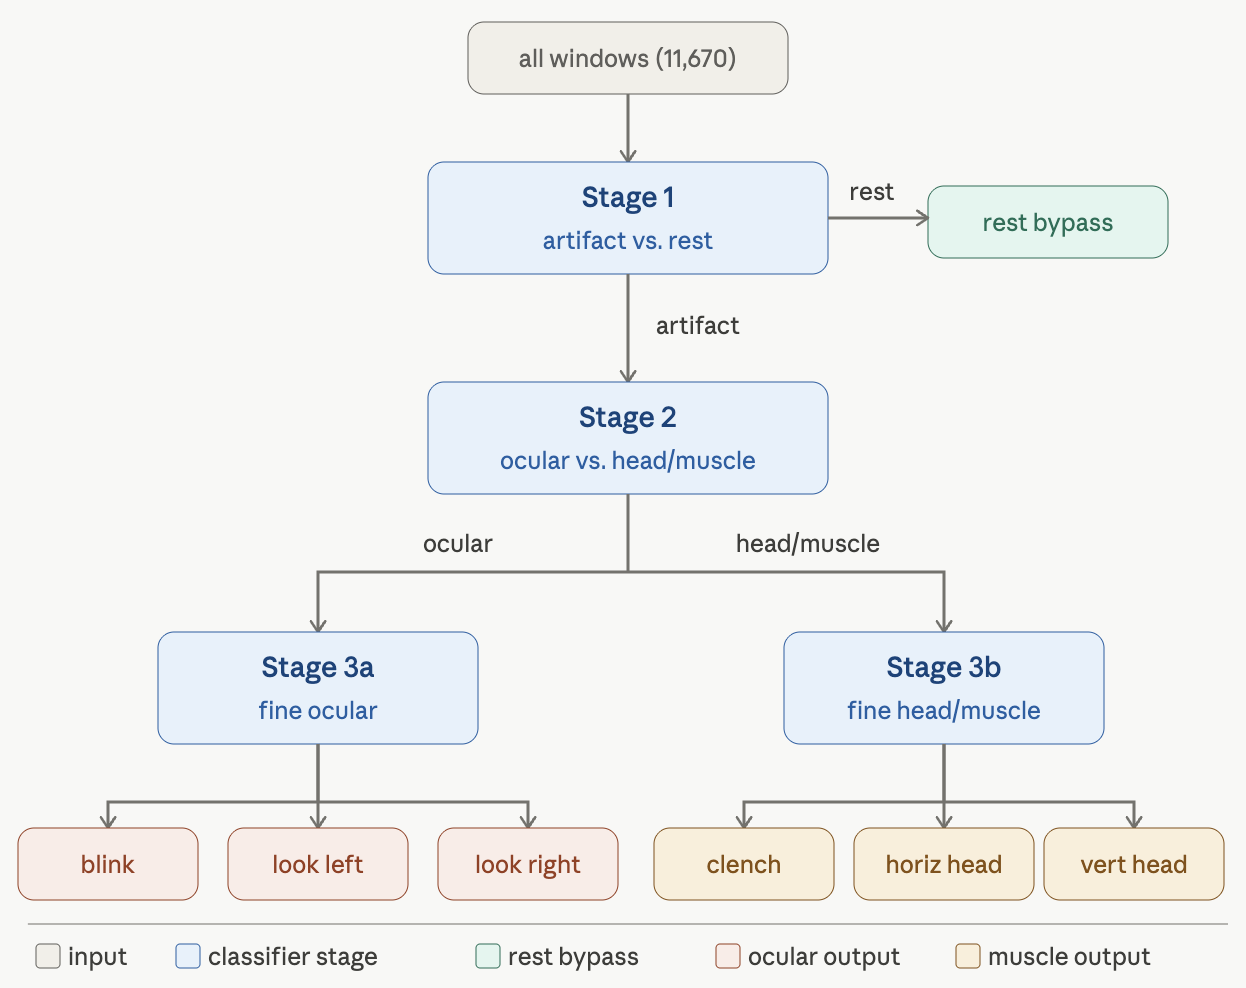
\includegraphics[width=0.95\columnwidth]{figures/Pipeline.png}
    \caption{Four-stage hierarchical classification pipeline.}
    \label{fig:pipeline}
\end{figure}

\subsection{Models Evaluated}
As a rule-based baseline, an amplitude thresholding classifier was evaluated on the binary Stage~1 task. Windows exceeding a subject-specific peak-to-peak threshold — optimised via grid search within each LOSO fold — were flagged as artifact; all others retained as rest.

Four model families were then benchmarked under identical LOSO conditions across all four hierarchical stages:

\begin{itemize}
    \item \textbf{Random Forest \& XGBoost:} Tree-based ensemble methods operating on the 324-dimensional handcrafted feature matrix, directly encoding domain knowledge through explicit frequency and morphological descriptors.

    \item \textbf{EEGNet:} A compact convolutional network combining temporal convolutions that simulate bandpass filtering with depthwise spatial convolutions across the 4 hardware channels. Per-layer max-norm regularisation controls overfitting under limited data.

    \item \textbf{1D-CNN:} Three sequential Conv1d blocks with BatchNorm and ReLU activations, followed by Adaptive GlobalMaxPooling and a dense classification head. GlobalMaxPooling is preferred over GlobalAveragePooling because artifacts are sparse transient events that may occur at any temporal position within a 2-second window.
\end{itemize}

Both neural networks were implemented in PyTorch, trained with Focal Loss ($\gamma = 2.0$) to address class imbalance. The per-fold per-channel z-score normalization was applied using statistics fitted to the training data only, preventing leakage into the test fold. Early stopping with patience of 15 epochs on validation macro F1 was enforced to prevent overfitting.


\subsection{LOSO Validation and Class Balancing}
In each of the 13 LOSO folds, all windows from the held-out subject form the test set $\mathcal{D}_{\text{test}}$; classifiers are trained from scratch on the pooled remaining 12 subjects ($\mathcal{D}_{\text{train}}$), preventing inter-subject data leakage. Class imbalance was addressed per model family: rest windows were downsampled for Stage~1 tree models; inverse-frequency class weights were applied across all tree stages; Focal Loss inherently suppresses gradient contributions from well-classified majority examples for neural networks.

\subsection{Model Interpretability}
\label{sec:xai}
To verify that classifier decisions align with underlying physiology, feature importance was aggregated across LOSO folds for the final XGBoost pipeline, and complementary SHAP analysis was conducted on a held-out subject. The top-10 features per stage are reported in Figure~\ref{fig:importance} (Appendix), confirming a clear stage-dependent structure. Stage~1 is dominated by amplitude and energy descriptors on real channels (delta-band power, peak-to-peak trajectory, variance), consistent with the binary task of separating high-energy artifact windows from low-amplitude rest. Stage~2 is entirely driven by virtual differential channels — particularly gamma-band trajectory asymmetries between anterior and posterior pairs — with no real channel appearing in the top~20, confirming that the ocular vs.\ head/muscle split is fundamentally a lateralisation and spectral asymmetry problem. Stage~3a relies on both anterior and posterior left-right asymmetries (diff\_Fp1\_Fp2 and diff\_F7\_F8 descriptors) alongside amplitude variance, reflecting the bilateral spatial signature of saccade direction. Stage~3b is led by spectral entropy on the anterior-posterior gradient and zero crossing rate on posterior asymmetry, with gamma-band power appearing from rank~3 onward — consistent with the difficulty of separating clench from head motion using spectral shape rather than raw power. For the EEGNet model, Grad-CAM confirmed that convolutional attention localised onto high-amplitude artifact segments rather than background noise.

\section{Signal-Domain \& Learned Denoising}
\label{sec:denoising}

\subsection{Wavelet, ASR and Cascade}
When Stage~1 flags a window as artifact, the pipeline conditionally triggers one of four denoising methods. ICA is excluded as it requires higher spatial rank than the 4-channel configuration provides; instead, the framework combines single-channel and subspace decomposition approaches:

\begin{enumerate}
    \item \textbf{Discrete Wavelet Transform (DWT):} Each window is decomposed using a \texttt{db4} mother wavelet at Level~5. High-frequency EMG content is attenuated across the detail sub-bands via soft-thresholding with threshold $\sigma\sqrt{2\ln N}$, where $N$ denotes the total number of time-domain window samples ($N=500$) and $\sigma$ is estimated from the finest-scale coefficients via the Median Absolute Deviation (MAD). The approximation sub-band is left untouched; the signal is reconstructed via the inverse DWT.

    \item \textbf{Artifact Subspace Reconstruction (ASR):} Each window is projected onto the subspace spanned by the subject's clean resting EEG. Calibration statistics are estimated from the subject's own rest windows (first and last 30~seconds of the recording, selected to mitigate baseline drift). Windows are decomposed via PCA; components exceeding $k=9$ times the clean-baseline variance are identified as artifact and reconstructed from the remaining clean subspace.

    \item \textbf{Cascaded DWT-ASR:} The raw window is first passed through DWT soft-thresholding to attenuate high-frequency EMG content, then routed through ASR to suppress residual low-frequency deflections, addressing mixed-mode artifact profiles across both frequency domains.
\end{enumerate}

\subsection{Residual 1D Convolutional Autoencoder}
As a learned alternative, a residual 1D convolutional autoencoder was trained for artifact subtraction. Rather than reconstructing the clean signal directly, the network estimates the artifact component, which is explicitly subtracted:
$$x_{\text{cleaned}} = x - \mathcal{D}\!\left(\mathcal{E}(x)\right)$$
The encoder compresses the 4-channel input via two strided Conv1d layers (stride~2 each); the decoder reconstructs via two ConvTranspose1d layers, producing a residual estimate at the original resolution. The network is trained with MSE loss against each subject's mean rest window as the clean target. A global normalisation fitted on rest windows only is applied before training and reversed after inference.

\section{Results \& Performance Evaluation}
\label{sec:results}

\subsection{Hierarchical Classification Performance}
The hierarchical classification pipeline was evaluated under strict LOSO cross-validation across all 13 subjects. Table~\ref{tab:model_comparison} reports chained macro $F_1$ scores for all models. The thresholding baseline operates only on the binary Stage~1 task and is not directly comparable to the chained 7-class scores of the other models.

\begin{table}[H]
\centering
\caption{Cross-model performance comparison (LOSO aggregate). Thresholding operates on Stage~1 only (binary); all other models report 7-class chained macro $F_1$.}
\label{tab:model_comparison}
\resizebox{\columnwidth}{!}{%
\begin{tabular}{lccc}
\hline
\textbf{Model} & \textbf{Input} & \textbf{Accuracy} & \textbf{Macro $F_1$} \\
\hline
Thresholding (Stage~1 only) & Raw windows    & 0.7759 & 0.7706 \\
Flat XGBoost (7-class)      & Feature matrix & 0.7530 & 0.6522 \\
Chained Random Forest       & Feature matrix & 0.7259 & 0.6196 \\
Chained EEGNet              & Raw windows    & 0.6835 & 0.5711 \\
Chained 1D-CNN              & Raw windows    & 0.7188 & 0.6196 \\
\textbf{Chained XGBoost}    & \textbf{Feature matrix} &
\textbf{0.7499} & \textbf{0.6576} \\
\hline
\end{tabular}%
}
\end{table}

The hierarchical XGBoost pipeline achieved the highest chained macro $F_1$ of 0.658, outperforming all deep temporal architectures. The per-stage breakdown (Figure~\ref{fig:confusion_matrices}) reveals distinct difficulty levels across the hierarchy:

\begin{itemize}
    \item \textbf{Stage 1 (artifact vs.\ rest):} Macro $F_1 = 0.881$, demonstrating reliable detection of contaminated windows.\item \textbf{Stage 2 (ocular vs.\ head/muscle):} Macro $F_1 = 0.935$, the strongest result across all stages, reflecting the large amplitude and frequency separation between the two groups. 
    \item \textbf{Stage 3a (fine ocular):} Macro $F_1 = 0.831$, with \texttt{look\_right} achieving the highest individual recall (0.87) and \texttt{blink} the lowest (0.81), with its primary confusion directed toward both saccade classes.
    \item \textbf{Stage 3b (fine head/muscle):} Macro $F_1 = 0.692$, the consistent bottleneck across all models. \texttt{horiz\_head} and \texttt{vert\_head} exhibit systematic confusion due to their indistinguishable frontal-temporal amplitude profiles — a hardware constraint rather than a modelling failure.
\end{itemize}

\begin{figure}[H]
    \centering
    \begin{subfigure}[t]{0.48\columnwidth}
        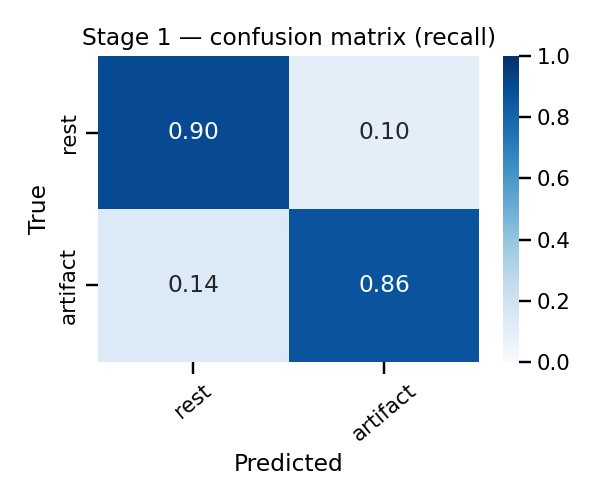
\includegraphics[width=\linewidth]{figures/xgb_stage1_confusion}
        \caption{Stage~1: artifact vs.\ rest.}
        \label{fig:cm_s1}
    \end{subfigure}
    \hfill
    \begin{subfigure}[t]{0.48\columnwidth}
        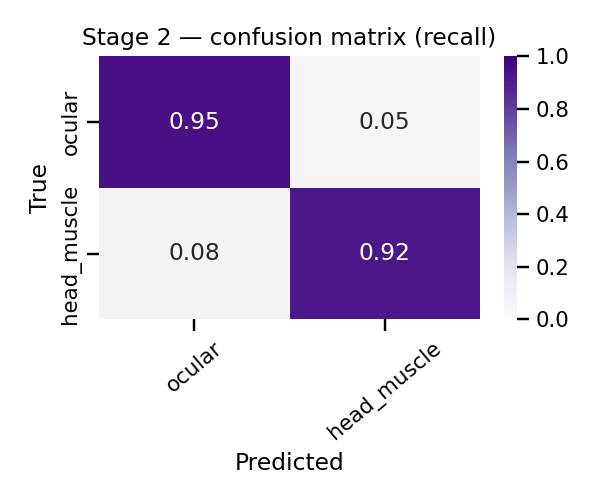
\includegraphics[width=\linewidth]{figures/xgb_stage2_confusion}
        \caption{Stage~2: ocular vs.\ head/muscle.}
        \label{fig:cm_s2}
    \end{subfigure}

    \vspace{0.5em}

    \begin{subfigure}[t]{0.48\columnwidth}
        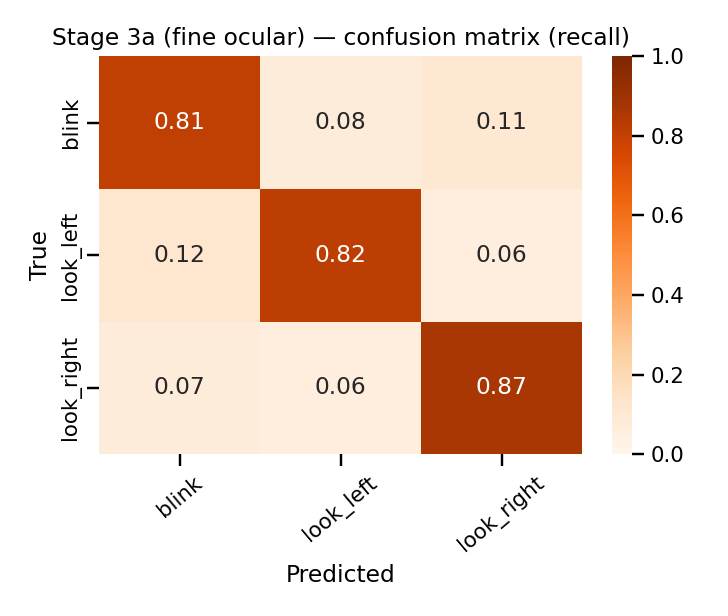
\includegraphics[width=\linewidth]{figures/xgb_stage3a_confusion}
        \caption{Stage~3a: fine ocular.}
        \label{fig:cm_s3a}
    \end{subfigure}
    \hfill
    \begin{subfigure}[t]{0.48\columnwidth}
        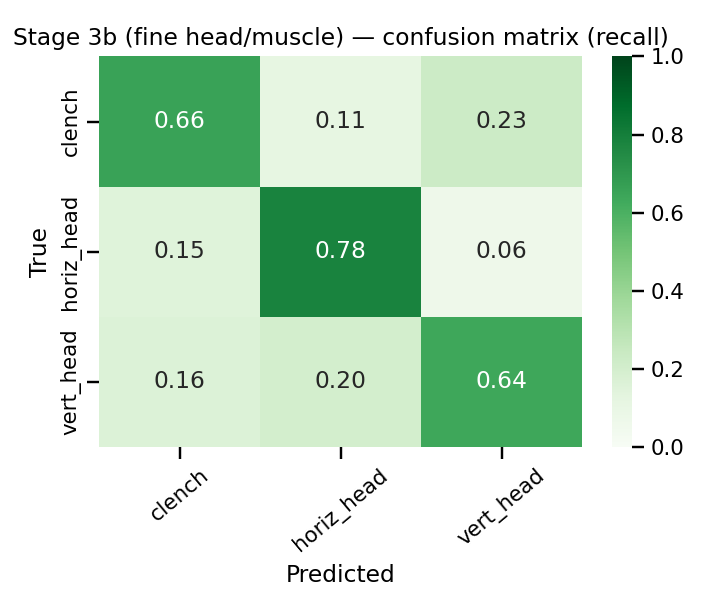
\includegraphics[width=\linewidth]{figures/xgb_stage3b_confusion}
        \caption{Stage~3b: fine head/muscle.}
        \label{fig:cm_s3b}
    \end{subfigure}
    \caption{Per-stage normalised recall confusion matrices for the chained XGBoost pipeline (LOSO aggregate, 13 subjects).}
    \label{fig:confusion_matrices}
\end{figure}

Inter-subject variability in Stage~1 detection was notable (per-subject $F_1$ standard deviation = 0.068, range 0.689--0.968), with the weakest subject nearly 0.28 $F_1$ points below the strongest, confirming that generalisation to unseen subjects remains the primary challenge for low-density wearable EEG systems.

\subsection{Denoising Performance}
\label{sec:denoising_results}
Four denoising methods were evaluated against per-subject rest baselines using artifact-band attenuation (dB), SNR improvement (dB), and RMS reduction (dB). Because no ground-truth clean cortical signal exists during active artifact trials, all metrics are computed relative to each subject's own rest window statistics.

\begin{table}[H]
\centering
\caption{Artifact-band attenuation (dB) per method and artifact class. Artifact band: 0.5--8~Hz for ocular and head movement classes; 30--99~Hz for clench. Negative values (italicised) indicate increased power. Bold marks the best result per class.}
\label{tab:denoising_metrics}
\resizebox{\columnwidth}{!}{%
\begin{tabular}{lcccc}
\hline
\textbf{Artifact class} & \textbf{Wavelet} & \textbf{ASR} &
\textbf{Wavelet+ASR} & \textbf{Autoencoder} \\ \hline
Blink       & 0.31 &  4.20 &  4.72 & \textbf{9.19}  \\
Look left   & 0.26 &  7.20 &  7.68 & \textbf{10.92} \\
Look right  & 0.28 &  4.91 &  5.42 & \textbf{10.45} \\
Horiz head  & 0.20 &  9.93 & 10.40 & \textbf{11.87} \\
Vert head   & 0.10 & 10.79 & 11.09 & \textbf{12.08} \\
Clench      & 10.0  &  2.93 & \textbf{12.29} & \textit{$-$2.95} \\
\hline
\textbf{Mean} & 1.86 & 6.66 & \textbf{8.60} & 8.59 \\ \hline
\end{tabular}%
}
\end{table}


In terms of overall signal-to-noise ratio enhancement, the pipeline yielded a mean SNR improvement of 0.18~dB for Wavelet, 5.11~dB for ASR, 5.34~dB for Wavelet+ASR, and 4.78~dB for the Autoencoder. These variations in SNR reflect the highly complementary spectral behaviors of the four methods across distinct noise profiles.

Wavelet produced negligible attenuation on low-frequency ocular and head movement artifacts, whose energy resides in the approximation coefficients and is untouched by soft-thresholding. For jaw clench, Wavelet achieved 10.0~dB attenuation — the highest among standalone methods — by correctly extracting broadband EMG from the detail sub-bands. ASR showed the inverse profile: consistent attenuation across all ocular and head movement classes via subspace projection, but only 2.93~dB on clench, where its projection captures the low-frequency sustained muscle component without addressing the broadband EMG content in the 30--99~Hz artifact band. Wavelet+ASR achieved the highest mean attenuation (8.60~dB) and best clench result (12.29~dB) by pre-attenuating high-frequency content before subspace projection, addressing both spectral components of the clench. The autoencoder achieved the strongest attenuation on ocular artifacts but produced negative attenuation on jaw clench ($-$2.95~dB): its learned low-frequency subtraction template adds back power in the 30--99~Hz band when applied to clench windows.

Figure~\ref{fig:denoising_residuals} confirms these behaviours on representative windows.

\begin{figure}[h]
    \centering
    \begin{subfigure}[b]{\linewidth}
        \centering
        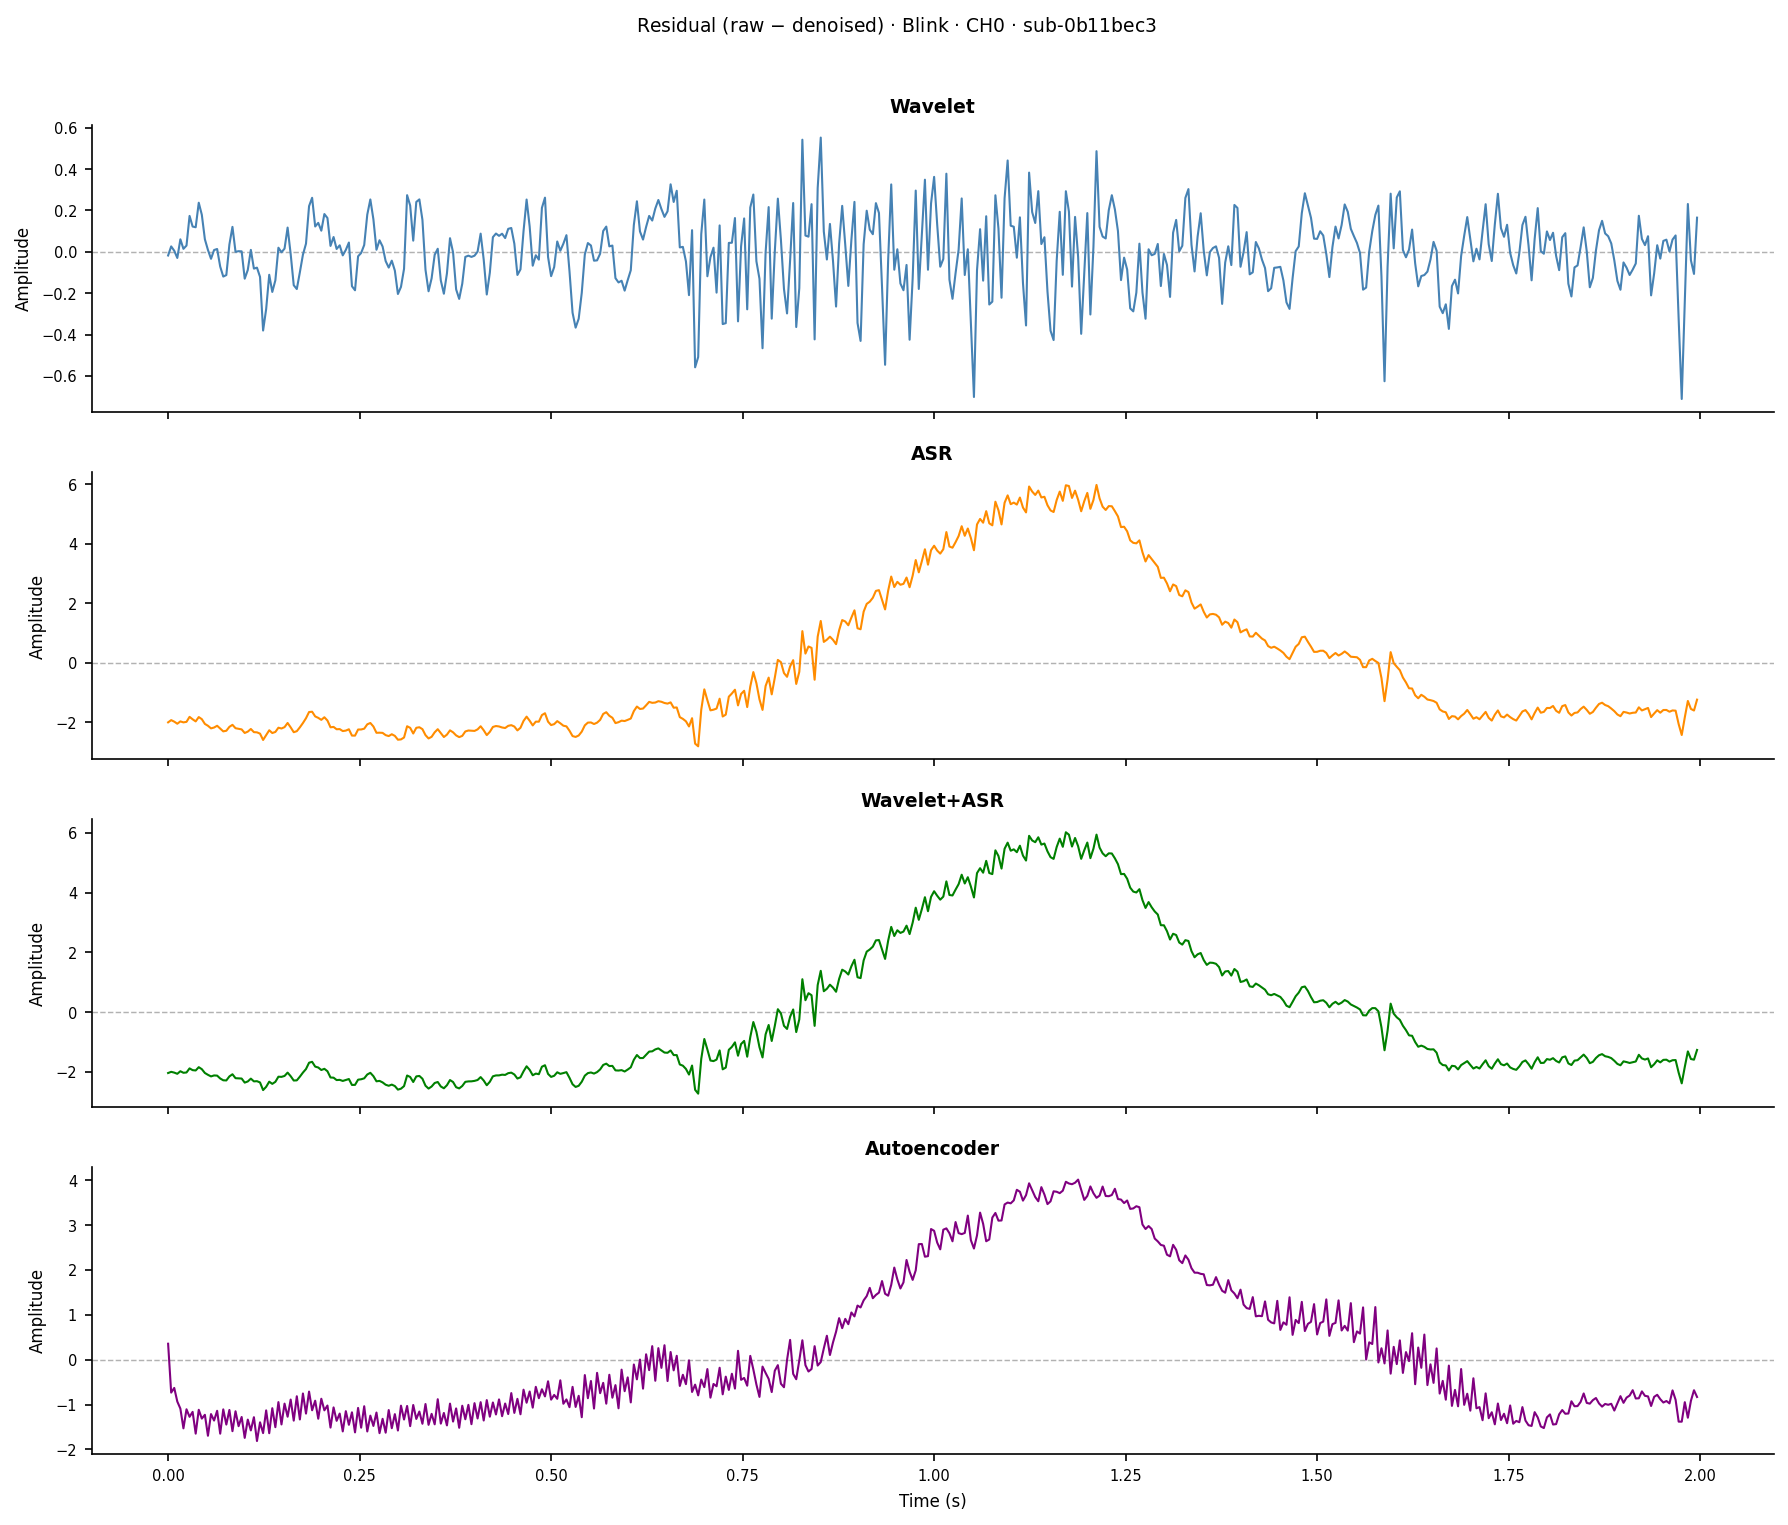
\includegraphics[width=0.8\linewidth]{figures/denoising_residuals_blink.png}
        \caption{Blink}
        \label{fig:denoising_blink}
    \end{subfigure}
    \vfill
    \begin{subfigure}[b]{\linewidth}
        \centering
        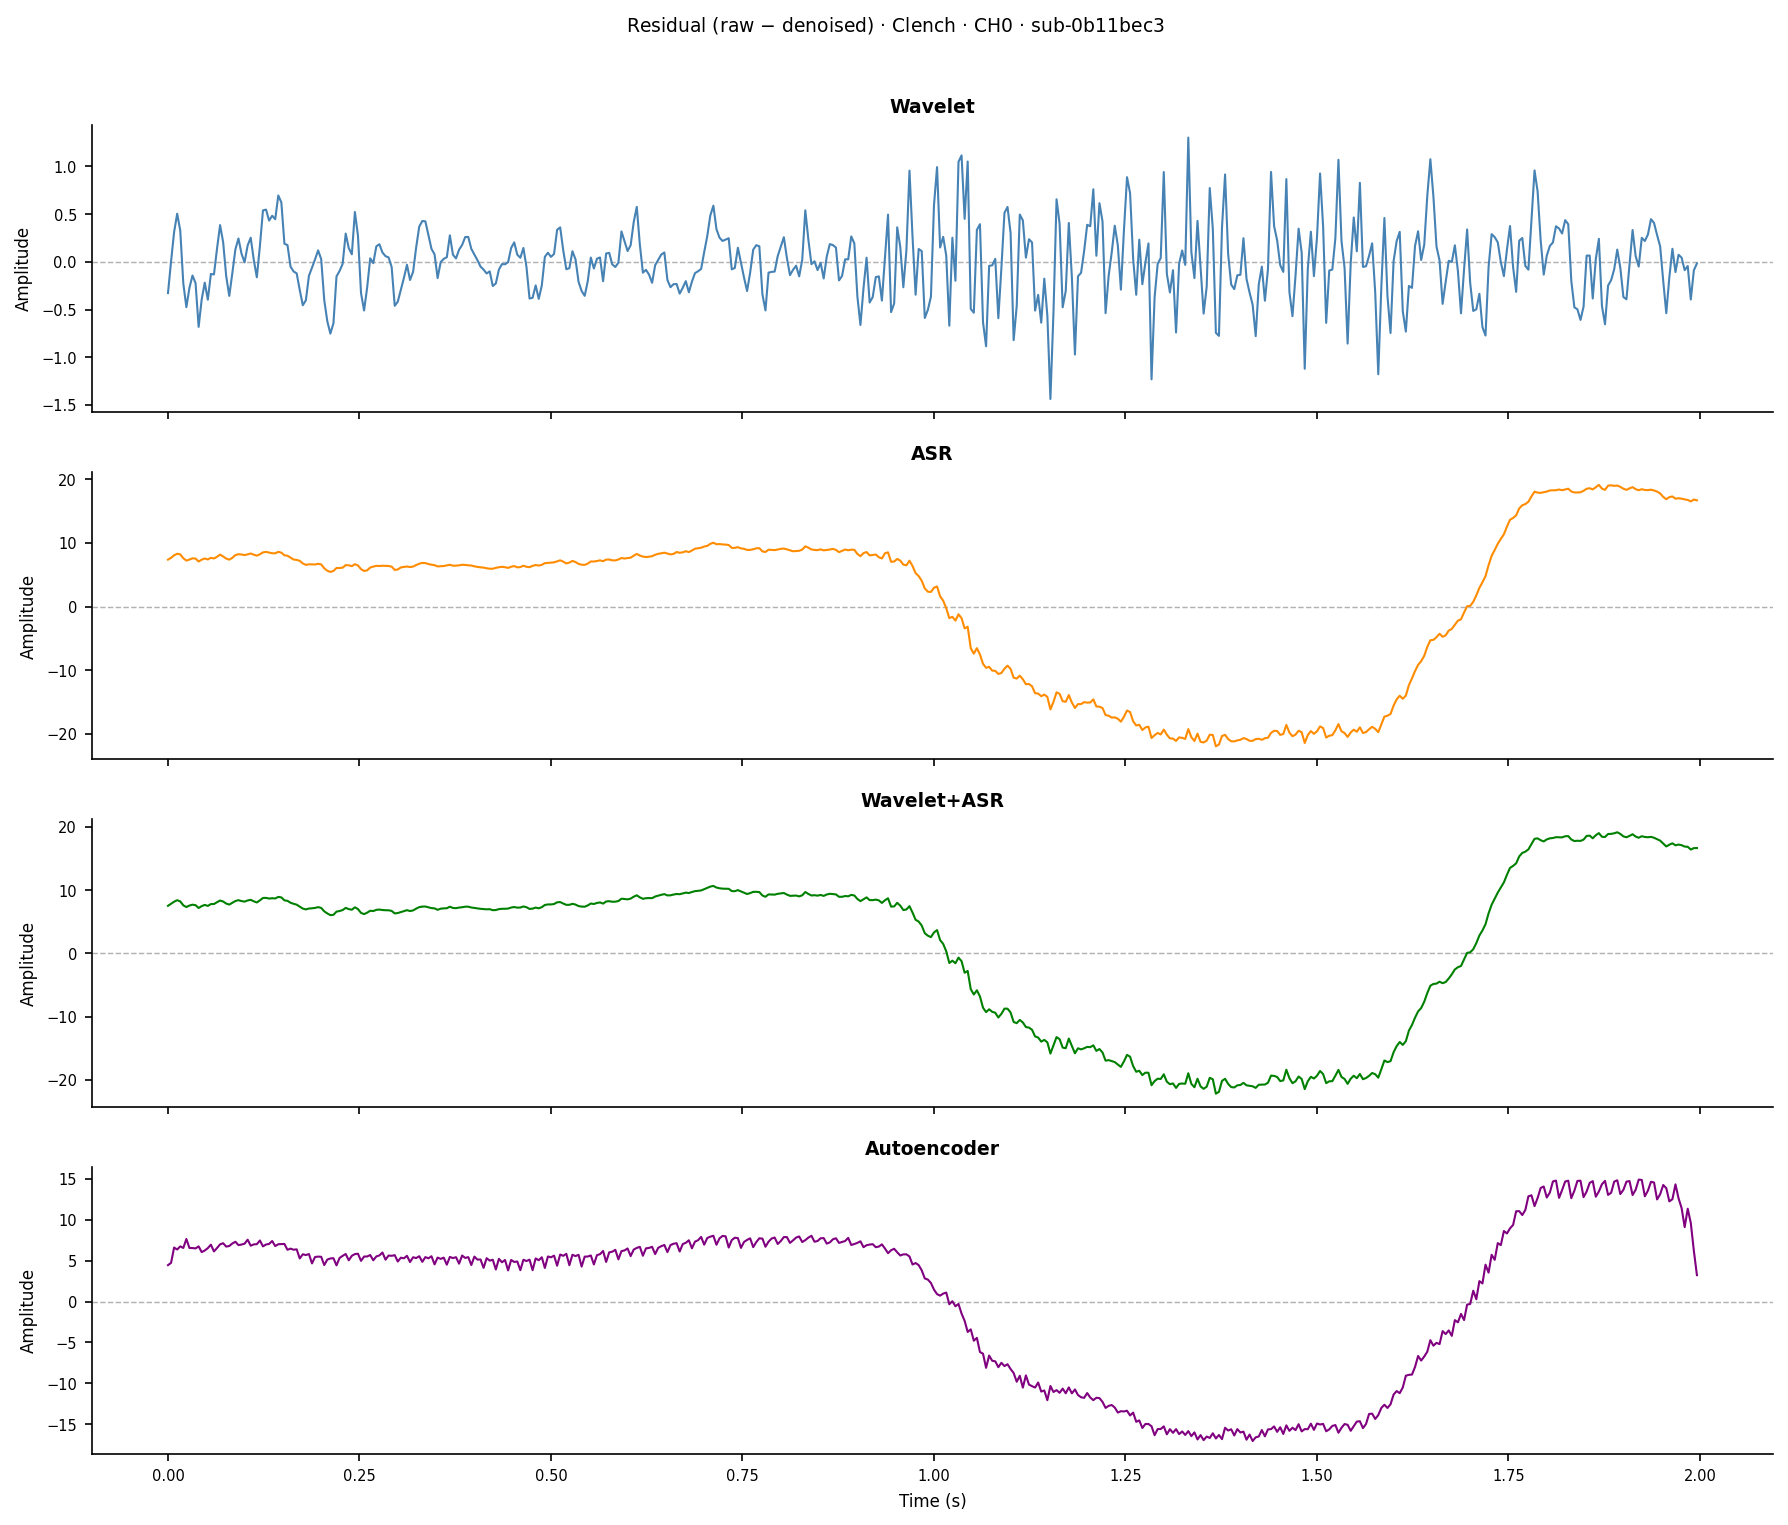
\includegraphics[width=0.8\linewidth]{figures/denoising_residuals_clench.png}
        \caption{Jaw clench}
        \label{fig:denoising_clench}
    \end{subfigure}
    \caption{Residual (raw $-$ denoised) on CH0 across all four methods for representative blink and jaw clench windows.}
    \label{fig:denoising_residuals}
\end{figure}

\subsection{Blind-Subject Evaluation}
The full pipeline was evaluated on a completely held-out subject. XGBoost was retrained on the remaining 12 subjects and Wavelet+ASR denoising was applied to all Stage~1 artifact-predicted windows.

\begin{table}[H]
\centering
\caption{Blind-subject evaluation vs.\ LOSO baseline (XGBoost, chained pipeline).}
\label{tab:blind_test}
\begin{tabular}{lcc}
\hline
\textbf{Stage} & \textbf{LOSO $F_1$} & \textbf{Blind $F_1$} \\ \hline
Stage 1   & 0.881 & 0.965 \\
Stage 2   & 0.935 & 0.998 \\
Stage 3a  & 0.831 & 0.891 \\
Stage 3b  & 0.692 & 0.505 \\
Chained   & 0.658 & 0.702 \\ \hline
\end{tabular}
\end{table}

Stages 1--3a generalised strongly to the unseen subject, with blind scores matching or exceeding the LOSO aggregate. Stage~3b dropped to $F_1 = 0.505$, consistent with the systematic \texttt{horiz\_head}/\texttt{vert\_head} confusion attributable to the electrode layout. The $\Delta$SNR comparison against the ground-truth upper bound is reported in Figure~\ref{fig:snr_comparison} (Appendix): the two pipelines are nearly identical except for blink, where Stage~1 misses a fraction of windows, reducing SNR improvement from 11.84~dB to 8.01~dB. Vertical head movements achieve the full theoretical 17.87~dB improvement since Stage~1 correctly routes all such windows to the denoiser regardless of their Stage~3b label.

\section{Discussion, Bonus Application, \& Conclusion}
\label{sec:discussion}

\subsection{Discussion}
The results confirm a clear performance advantage for handcrafted feature-based approaches over end-to-end deep temporal networks under the data constraints of this study. With only 12 training subjects per LOSO fold, deep architectures must rediscover from raw waveforms the frequency discriminators — broadband gamma power for clench, kurtosis for blink — that the 324-dimensional feature space encodes explicitly. The 4-channel spatial layout further limits the inter-channel covariance information available to convolutional layers. The hierarchical XGBoost pipeline achieved a chained macro $F_1$ of 0.658, outperforming the flat 7-class baseline (0.652) and confirming the benefit of decomposing the problem into targeted binary and ternary decisions.

Stage~2 ($F_1 = 0.935$) proved the easiest split across all models, reflecting the order-of-magnitude amplitude and frequency separation between ocular and musculoskeletal groups. Stage~3b ($F_1 = 0.692$) was the consistent bottleneck: the lateral temporal electrode placement provides no directional specificity for head rotation plane, making \texttt{horiz\_head} and \texttt{vert\_head} indistinguishable from frontal-temporal signals alone. This is a hardware constraint rather than a modelling failure — integration of an inertial measurement unit (IMU) would trivially resolve this class pair. The absence of a dedicated EOG reference channel similarly constrains denoising quality, as ocular artifacts share both their spatial origin and frequency band (0.5--8~Hz) with endogenous frontal neural rhythms.

For denoising, Wavelet+ASR achieved the most consistent broadband suppression (mean 8.60~dB), while the autoencoder's failure on jaw clench highlights the need for class-conditioned architectures in spectrally heterogeneous artifact datasets.

\subsection{Proposed Application: Hybrid Brain-Computer Interface}
The multi-stage classification output provides a natural foundation for a hybrid Brain-Computer Interface (BCI). Rather than discarding detected artifacts, stereotyped intentional patterns — voluntary blinks or jaw clenches — can be routed to an auxiliary control interface as discrete operational commands, while the parallel Wavelet+ASR stream outputs clean cortical time-series for downstream cognitive tracking. This dual-path architecture would convert physiological interference into an asset, increasing communication bandwidth for low-density wearable systems without compromising neural signal integrity.

\subsection{Conclusion}
This work presented a complete pipeline for multi-class EEG artifact classification and denoising on a 4-channel wearable headset. The four-stage hierarchical XGBoost architecture achieved the best chained macro $F_1$ of 0.658 under strict LOSO cross-validation. The primary bottleneck — Stage~3b discrimination of horizontal versus vertical head movements — is rooted in electrode placement and resolvable with IMU integration. Wavelet+ASR provided the most consistent denoising across artifact classes, while the autoencoder excelled on ocular artifacts but failed spectrally on jaw clench. Blind-subject evaluation confirmed generalisation at a chained $F_1$ of 0.702, with up to 17.87~dB SNR improvement on head movement artifacts.

\bibliographystyle{acl_natbib}
\begin{thebibliography}{}
\bibitem[{Chen \& Guestrin(2016)}]{xgboost}
Chen, T., \& Guestrin, C. (2016).
\newblock {XGBoost}: A scalable tree boosting system.
\newblock In \emph{Proceedings of the 22nd ACM SIGKDD International Conference on Knowledge Discovery and Data Mining} (pp. 785--794).
\bibitem[{Lawhern et~al.(2018)Lawhern, Solon, Waytowich, Gordon, Hung, \& Chou}]{eegnet}
Lawhern, V.~J., Solon, A.~J., Waytowich, N.~R., Gordon, S.~M., Hung, C.~P., \& Chou, P.~S. (2018).
\newblock {EEGNet}: a compact convolutional neural network for EEG-based brain--computer interfaces.
\newblock \emph{Journal of Neural Engineering}, 15(5), 056013.
\bibitem[{Mullen et~al.(2015)Mullen, Kothe, Chi, Ojeda, Kerth, Makeig, \& Cauwenberghs}]{asr}
Mullen, T.~R., Kothe, C.~A., Chi, Y.~M., Ojeda, A., Kerth, T., Makeig, S., \& Cauwenberghs, G. (2015).
\newblock Real-time neuroimaging and cognitive monitoring using wearable dry-EEG.
\newblock In \emph{2015 37th Annual International Conference of the IEEE Engineering in Medicine and Biology Society (EMBC)} (pp. 4222--4225). IEEE.
\end{thebibliography}

\appendix

\begin{figure*}[h]
    \centering
    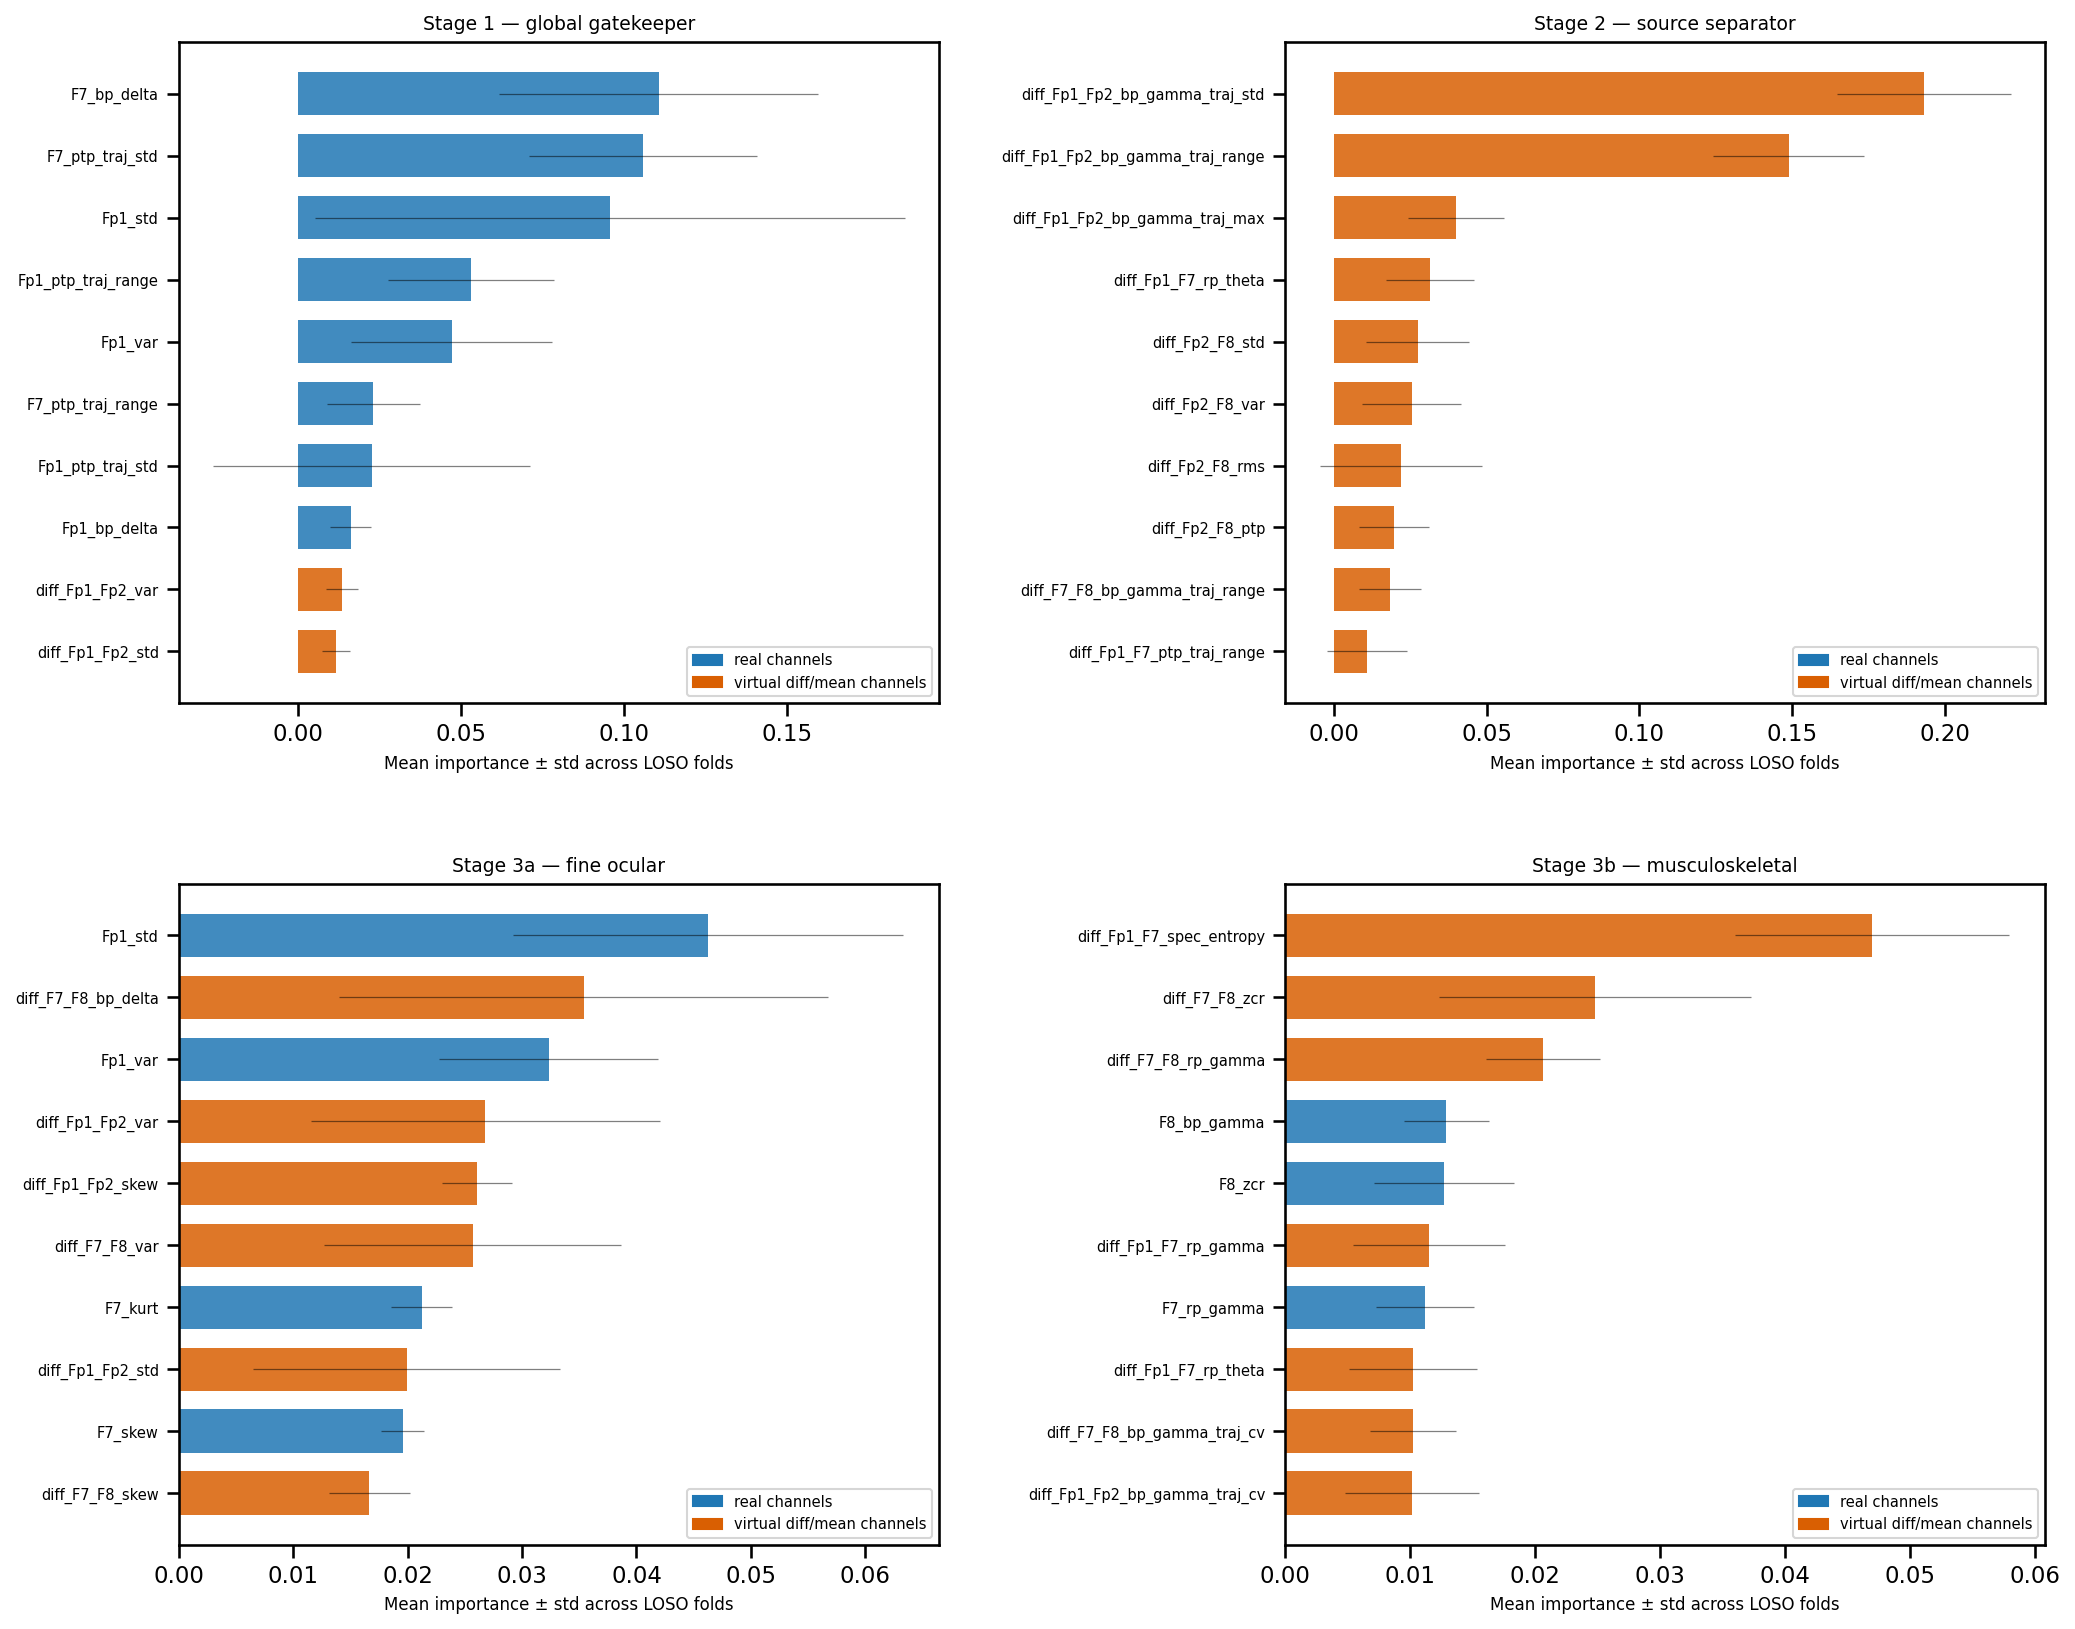
\includegraphics[width=\textwidth]{figures/feature_importance_grid.png}
    \caption{Top-10 XGBoost feature importances per stage (mean $\pm$ std across 
    LOSO folds). Blue: real hardware channels. Orange: virtual differential/mean 
    channels. The progressive shift from amplitude descriptors (Stage~1) to 
    asymmetry and spectral shape features (Stages~2--3b) reflects the increasing 
    discrimination difficulty at each level of the hierarchy.}
    \label{fig:importance}
\end{figure*}

\begin{figure*}[h]
    \centering
    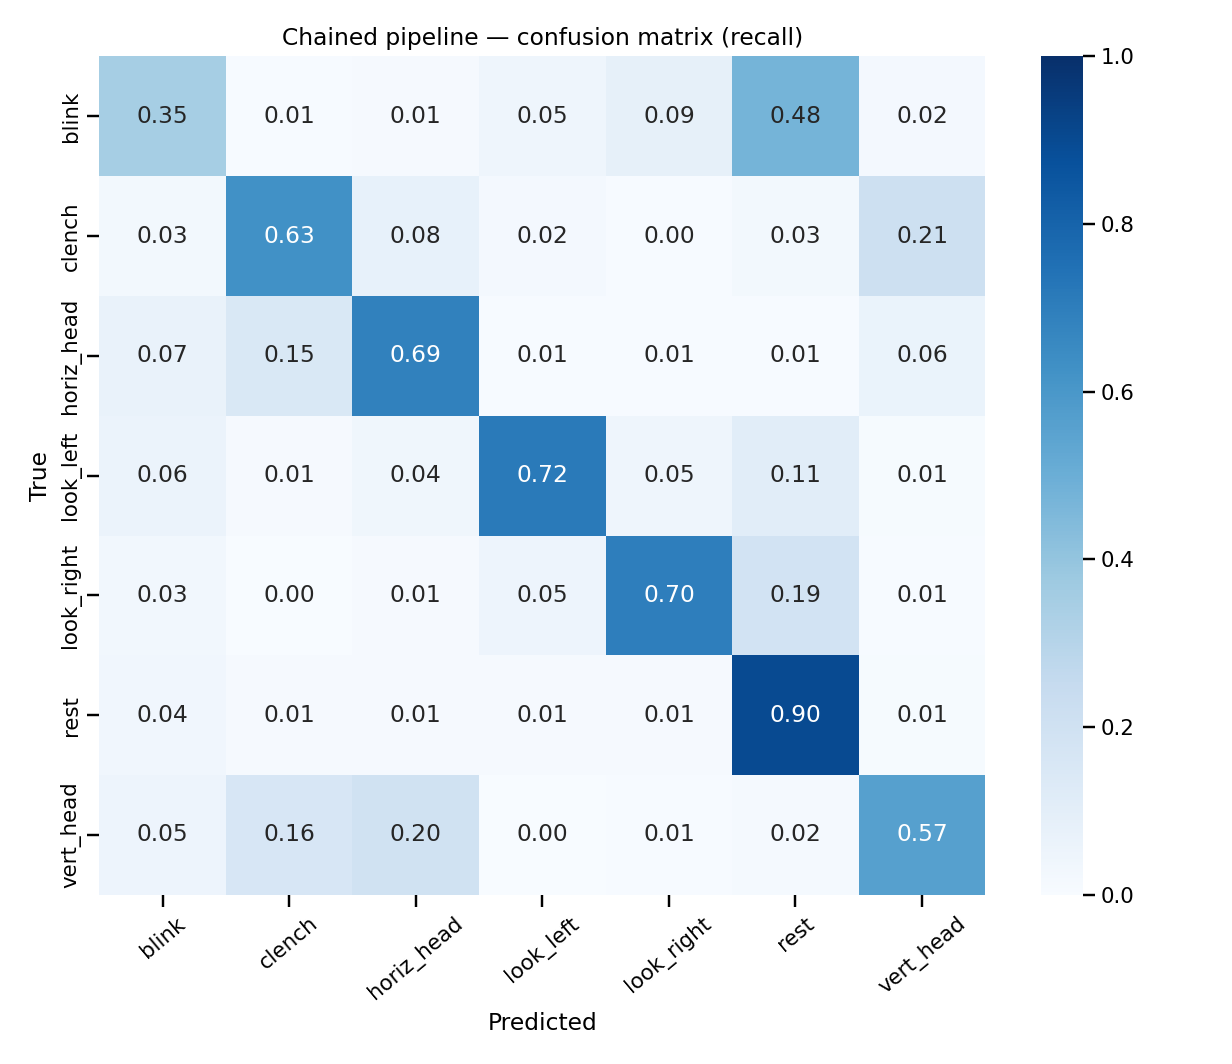
\includegraphics[width=0.6\textwidth]{figures/xgb_chained_confusion}
    \caption{Normalised recall confusion matrix for the full 
    7-class chained XGBoost pipeline (LOSO aggregate, 13 subjects).}
    \label{fig:chained_confusion}
\end{figure*}

\begin{figure*}[h]
    \centering
    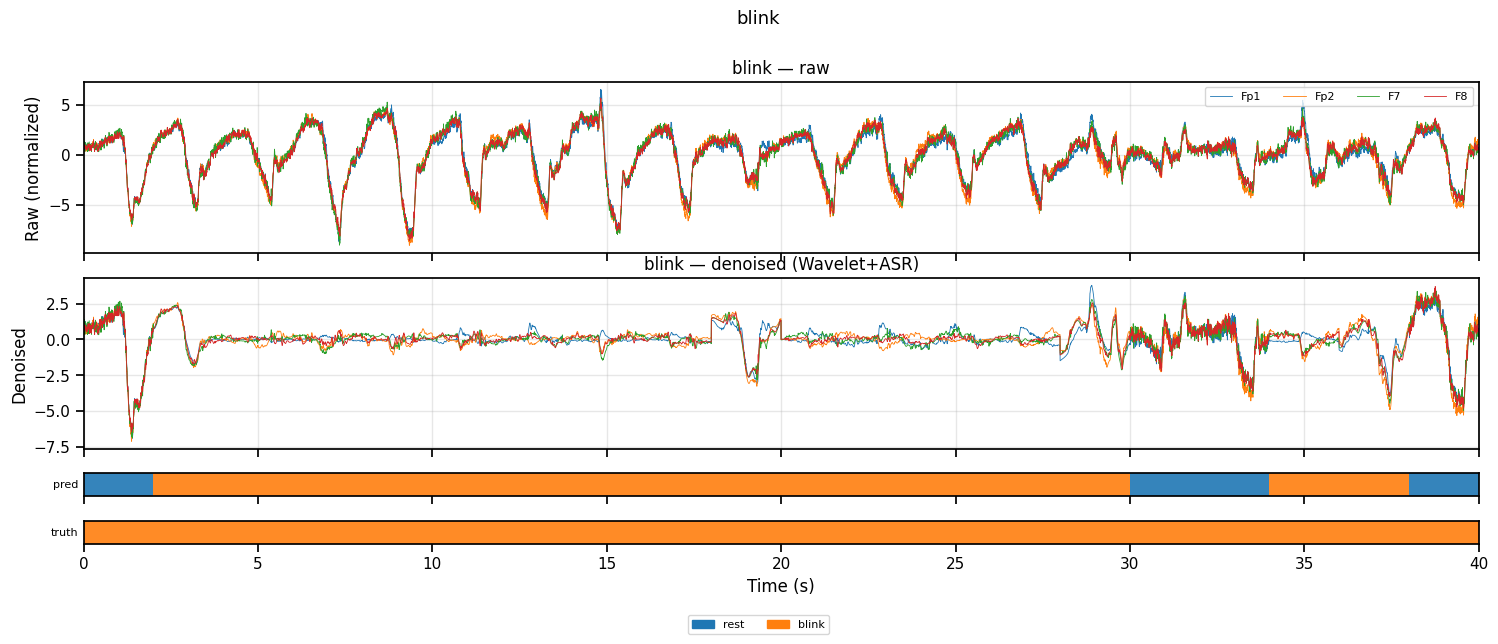
\includegraphics[width=\textwidth]{figures/eeg_blink_reconstruction.png}
    \caption{Continuous EEG reconstruction and artifact removal for the blinking task. 
    The top panel displays the normalized raw EEG data across four frontal channels, capturing prominent ocular artifacts. 
    The second panel shows the denoised continuous signal, where windows predicted as artifacts are replaced by the Wavelet+ASR pipeline output, while rest-predicted windows remain raw. 
    The bottom narrow annotation strips indicate the window-by-window classifier predictions (\textit{pred}) and the actual ground truth (\textit{truth}), color-coded by class (blue for rest, orange for blink).}
    \label{fig:eeg_blink_reconstruction}
\end{figure*}

\begin{figure*}[h]
    \centering
    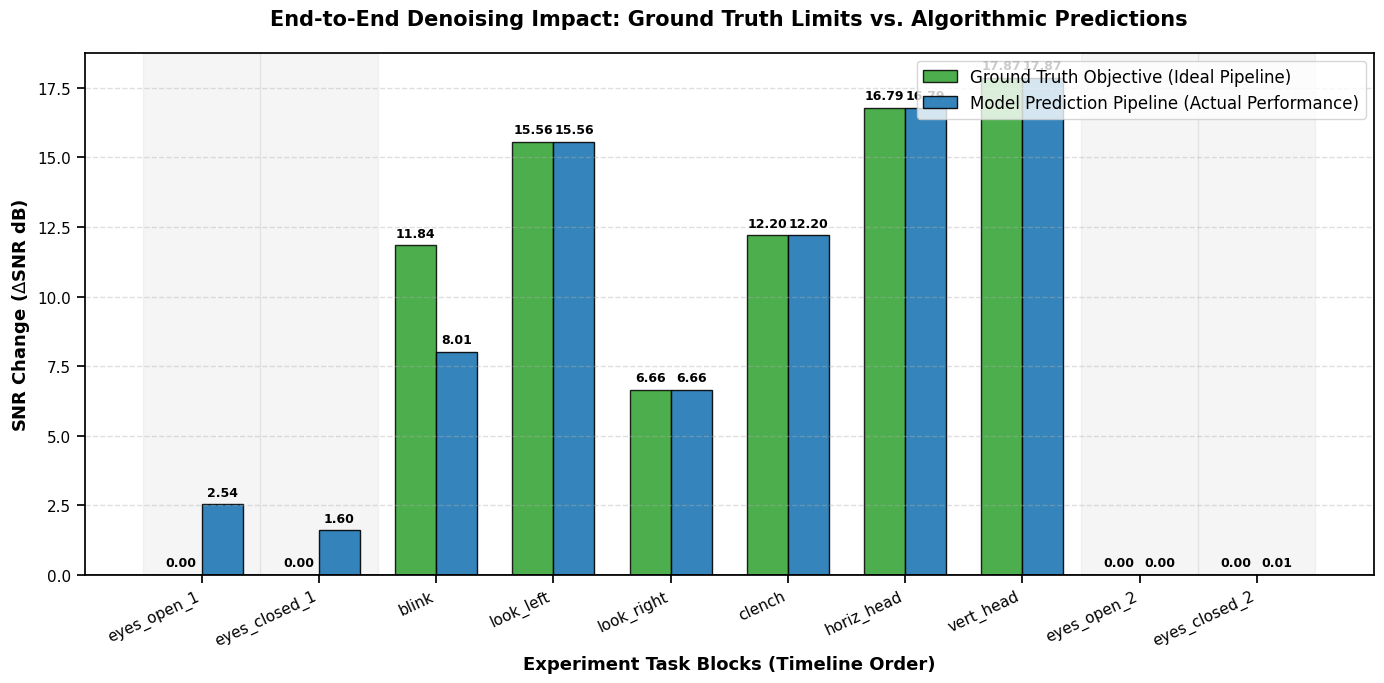
\includegraphics[width=\textwidth]{figures/snr_ground_truth_vs_prediction}
    \caption{$\Delta$SNR improvement (dB) per task block comparing 
    the ground-truth upper bound (green) against the model 
    prediction pipeline (blue). The blink gap (11.84~dB 
    vs.\ 8.01~dB) reflects Stage~1 missed detections. Vertical 
    head movements achieve the full theoretical 17.87~dB 
    improvement despite Stage~3b label confusion, since Stage~1 
    correctly routes all such windows to the denoiser regardless 
    of fine-grained label.}
    \label{fig:snr_comparison}
\end{figure*}



\end{document}